% !TEX program = xelatex
% ============================================================
%  翻译项目总装入口
%  编译：latexmk -xelatex（或运行 scripts/build.ps1）
% ============================================================
\documentclass[UTF8, fontset=none, twoside, openright, 11pt]{ctexbook}

% 由 scripts/prepare.py 从 project.json 生成，请勿手改
\newcommand{\booktitle}{中文书名}
\newcommand{\booksubtitle}{中文副题（可留空）}
\newcommand{\booktitleoriginal}{Original Title}
\newcommand{\booksubtitleoriginal}{Original Subtitle}
\newcommand{\bookauthor}{作者中文名}
\newcommand{\bookauthororiginal}{Author Name}
\newcommand{\booktranslator}{（译者姓名）}
\newcommand{\bookseries}{}
\newcommand{\bookpublisher}{}
\newcommand{\bookoriginalpublisher}{}
\newcommand{\bookoriginalyear}{}
\newcommand{\bookyear}{2026}
\newcommand{\bookversion}{0.1}
\newcommand{\bookrights}{待确认}
\newcommand{\bookkeywords}{翻译; 书籍}
      % 由 project.json 生成，勿手改
% ============================================================
%  翻译工作区 · 通用排版导言区
%  引擎：XeLaTeX（必须）
%  项目专用改动请写在 project.tex 或正文中，尽量不改本文件
% ============================================================

% ---------- 宏包 ----------
\usepackage{geometry}
\usepackage{fancyhdr}
\usepackage{enumitem}
\usepackage{booktabs}
\usepackage{longtable}
\usepackage{array}
\usepackage{tabularx}
\usepackage{multirow}
\usepackage{graphicx}
\usepackage{xcolor}
\usepackage{float}
\usepackage{setspace}
\usepackage{ragged2e}
\usepackage{caption}
\usepackage{tocloft}
\usepackage{amsmath,amssymb}
\usepackage{microtype}

% ---------- 页面 ----------
\geometry{
  paperwidth=170mm,
  paperheight=240mm,
  top=25mm,
  bottom=25mm,
  inner=22mm,
  outer=18mm,
  headheight=14pt,
  headsep=6mm,
  footskip=12mm
}

% ---------- 字体 ----------
% 西文：Palatino（正文），Consolas（等宽）
\setmainfont{Palatino Linotype}[
  BoldFont={Palatino Linotype Bold},
  ItalicFont={Palatino Linotype Italic},
  BoldItalicFont={Palatino Linotype Bold Italic}
]
\setsansfont{Segoe UI}
\setmonofont{Consolas}[Scale=MatchLowercase]

% 中文：Noto Serif SC（正文）、Noto Sans SC（标题/无衬线）、楷体、仿宋
% 注：系统安装的 Noto SC 为可变字体（VF），xdvipdfmx 无法嵌入，
% 故正文用宋体、标题用黑体；两者均为 Windows 自带、可稳定嵌入。
% 如安装了静态版思源宋体/黑体，可改为 Source Han Serif SC / Source Han Sans SC。
\setCJKmainfont{SimSun}[AutoFakeBold=1.5]
\setCJKsansfont{SimHei}
\setCJKmonofont{FangSong}
\setCJKfamilyfont{zhsong}{SimSun}[AutoFakeBold=1.5]
\setCJKfamilyfont{zhhei}{SimHei}
\setCJKfamilyfont{zhkai}{KaiTi}
\setCJKfamilyfont{zhfs}{FangSong}
\providecommand{\songti}{}
\providecommand{\heiti}{}
\providecommand{\kaishu}{}
\providecommand{\fangsong}{}
\renewcommand{\songti}{\CJKfamily{zhsong}}
\renewcommand{\heiti}{\CJKfamily{zhhei}}
\renewcommand{\kaishu}{\CJKfamily{zhkai}}
\renewcommand{\fangsong}{\CJKfamily{zhfs}}

% ---------- 行距与段落 ----------
\linespread{1.45}
\setlength{\parindent}{2em}
\setlength{\parskip}{0pt}
\setlength{\emergencystretch}{2em}

% ---------- 章节标题 ----------
\ctexset{
  chapter = {
    format = \centering,
    nameformat = \sffamily\large\bfseries,
    numberformat = \sffamily\large\bfseries,
    titleformat = \sffamily\LARGE\bfseries,
    name = {第,章},
    number = \chinese{chapter},
    beforeskip = 20pt,
    afterskip = 40pt
  },
  section = {
    format = \sffamily\large\bfseries,
    beforeskip = 1.4ex plus .3ex minus .2ex,
    afterskip = .8ex plus .2ex
  },
  subsection = {
    format = \sffamily\normalsize\bfseries,
    beforeskip = 1.2ex plus .2ex minus .1ex,
    afterskip = .6ex plus .1ex
  }
}
% 章首不显示页眉线，章标题页使用 plain 样式
\renewcommand{\chaptermark}[1]{\markboth{#1}{#1}}

% 空白页不显示页眉页脚（book 类默认会给空白页加页眉）
\makeatletter
\renewcommand{\cleardoublepage}{%
  \clearpage
  \if@twoside
    \ifodd\c@page\else
      \hbox{}\thispagestyle{empty}\newpage
      \if@twocolumn\hbox{}\newpage\fi
    \fi
  \fi}
\makeatother

% 目录、插图目录标题居中
\renewcommand{\contentsname}{\hfill 目\quad 录\hfill}
\renewcommand{\listfigurename}{\hfill 插图目录\hfill}

% ---------- 页眉页脚 ----------
\pagestyle{fancy}
\fancyhf{}
\fancyhead[LE]{\small\itshape\booktitle}
\fancyhead[RO]{\small\itshape\leftmark}
\fancyfoot[C]{\small\thepage}
\renewcommand{\headrulewidth}{0.4pt}
\renewcommand{\footrulewidth}{0pt}
\fancypagestyle{plain}{%
  \fancyhf{}%
  \fancyfoot[C]{\small\thepage}%
  \renewcommand{\headrulewidth}{0pt}%
}

% ---------- 脚注 ----------
\usepackage[bottom,hang,flushmargin]{footmisc}
\renewcommand{\footnotelayout}{\small}
% 原书脚注每章从 1 开始，与原文编号对应
\counterwithin*{footnote}{chapter}
\setlength{\skip\footins}{1.1\baselineskip}

% ---------- 引文 ----------
% 短引文：随文引号；长引文：quote 环境（自动缩进 + 小字号）
\renewenvironment{quote}
  {\list{}{\leftmargin=2em\rightmargin=2em}\item[]\small\kaishu}
  {\endlist}

% 章首题词（题词正文译出，出处保留原文）
% 用法：\begin{chapterquote}{——作者，\textit{书名}}
%          ……题词……
%       \end{chapterquote}
\newenvironment{chapterquote}[1]
  {\def\chapterquotesource{#1}\begin{quote}\kaishu\small}
  {\par\vspace{0.8em}\hfill\upshape\small\chapterquotesource\end{quote}}

% ---------- 表格 ----------
\renewcommand{\arraystretch}{1.25}
\setlength{\tabcolsep}{6pt}
\captionsetup[table]{position=top}

% ---------- 图注 ----------
\captionsetup{
  font=small,
  labelfont=bf,
  labelsep=quad,
  skip=6pt
}
\graphicspath{{figures/}{source/images/}}

% ---------- 列表 ----------
\setlist[itemize]{leftmargin=2em,itemsep=0.2ex,topsep=0.4ex}
\setlist[enumerate]{leftmargin=2em,itemsep=0.2ex,topsep=0.4ex}

% ---------- 译者工具宏 ----------
% 术语首次出现：中文（原文）
% 用法：\term{述行性}{performativity}
\newcommand{\term}[2]{#1（\textit{#2}）}

% 仅保留原文（限定为西文斜体）
\newcommand{\orig}[1]{\textit{#1}}

% 译者注：独立编号（每章重新计数），不占用原书脚注编号。
% 页脚显示“译者注1：……”，正文标记为“〔译注1〕”
% 用法：\zhu{……}
\newcounter{zhu}[chapter]
\newcommand{\zhu}[1]{%
  \stepcounter{zhu}%
  \textsuperscript{〔译注\thezhu〕}%
  \begingroup
  \renewcommand{\thefootnote}{}%
  \footnotetext{\textbf{译者注\thezhu：}#1}%
  \endgroup}


% 独立参考文献/原注中的书名等，避免过度排版
\newcommand{\bookorig}[1]{\textit{#1}}

% 待办标记：编译可见，终检前必须清零
\newcommand{\todo}[1]{\textcolor{red}{【TODO：#1】}}

% 译者按语（块级，带底纹）
\usepackage[breakable]{tcolorbox}
\newtcolorbox{transnote}[1][译者注]{
  breakable,
  colback=black!3,
  colframe=black!35,
  boxrule=0.4pt,
  arc=1.5pt,
  left=8pt,
  right=8pt,
  top=6pt,
  bottom=6pt,
  fonttitle=\small\sffamily\bfseries,
  title={#1},
  before skip=1.2ex,
  after skip=1.2ex
}

% 图注来源行
% 用法：\figsource{图片来源：某某出版社}
\newcommand{\figsource}[1]{\par\vspace{0.3em}{\footnotesize #1\par}}

% ---------- 目录 ----------
\renewcommand{\cftchapfont}{\sffamily\bfseries}
\renewcommand{\cftchappagefont}{\sffamily}
\setlength{\cftbeforechapskip}{0.6em}
\setlength{\cftsecindent}{2em}

% ---------- 超链接与 PDF 元数据 ----------
\usepackage[
  colorlinks=true,
  linkcolor=black,
  citecolor=black,
  urlcolor=blue!45!black,
  bookmarksnumbered=true,
  bookmarksopen=true,
  pdfencoding=auto
]{hyperref}
\hypersetup{
  pdftitle={\booktitle},
  pdfauthor={\bookauthor},
  pdfsubject={\booktitleoriginal},
  pdfkeywords={\bookkeywords},
  pdfcreator={XeLaTeX}
}

% ---------- 其他 ----------
            % 版式与宏

\begin{document}

% ---------------- 前置部分 ----------------
\frontmatter
\pagestyle{empty}
% 封面：简洁排印式。如需图片封面，改为 \includegraphics[width=\paperwidth]{...}
\begin{titlepage}
\centering
\vspace*{2.2cm}

{\sffamily\bfseries\fontsize{30}{38}\selectfont \booktitle\par}

\vspace{0.8cm}
{\sffamily\large \booksubtitle\par}

\vspace{1.4cm}
{\itshape\normalsize \booktitleoriginal\par}
\ifx\booksubtitleoriginal\empty\else
  {\itshape\small \booksubtitleoriginal\par}
\fi

\vfill

{\large \bookauthor\par}
\vspace{0.25cm}
{\small\itshape \bookauthororiginal\par}

\vfill

{\normalsize 译者　\booktranslator\par}
\vspace{0.8cm}
{\small \bookpublisher\par}
{\small \bookyear\par}

\vspace*{1.2cm}
\end{titlepage}


\newpage
\thispagestyle{empty}
% 版权与翻译说明页（页脚不显示页码，由 \thispagestyle{empty} 控制）
\vspace*{\fill}
\begin{center}
{\sffamily\bfseries 版权与翻译说明}
\end{center}
\vspace{1.5em}

{\small
\begin{spacing}{1.3}
\begin{flushleft}

原书书名：\textit{\booktitleoriginal}\\
原书作者：\bookauthororiginal\\
原书出版者：\bookoriginalpublisher\\
原书出版年：\bookoriginalyear\\
中文书名：\booktitle\\
中文副题：\booksubtitle\\
译者：\booktranslator\\
版本：\bookversion\\
年份：\bookyear

\vspace{1.2em}
\hrule
\vspace{1.2em}

版权状态：\bookrights

\vspace{0.8em}
本书中文译本的权利归属与使用范围，以版权状态说明及权利方授权为准。\\
原文中的引文、插图、表格等，其版权归原权利人所有；\\
如涉及第三方权利，以原书版权页与权利方要求为准。

\vspace{0.8em}
译文中的注释分为两类：原书脚注以普通脚注排印；\\
译者所加注释以“译者注”标明。

\vspace{1.2em}
\hrule
\vspace{1.2em}

如发现译文错误，欢迎通过项目维护渠道指正。\\
勘误将记录于项目 \texttt{notes/decisions.md}，并在再版时修订。

\end{flushleft}
\end{spacing}
}

\vspace*{\fill}


% 献词（若已翻译）
\IfFileExists{frontmatter/dedication.tex}
  {\cleardoublepage\input{frontmatter/dedication}}

\cleardoublepage
\pagestyle{fancy}
\chapter*{译者说明}
\addcontentsline{toc}{chapter}{译者说明}
\markboth{译者说明}{译者说明}

\begin{flushleft}

本书依据 \textit{\booktitleoriginal}（\bookauthororiginal\ 著）译出。译文力求贴近原文的论证层次与语气，同时按中文的阅读习惯调整句法；凡涉及作者核心概念、历史背景或双关之处，以脚注或“译者注”说明。

\vspace{0.6em}
\textbf{关于术语。}全书人名、地名、机构名与学术术语原则上从通行译法；同一概念只用一个译名。首次出现时以“中文（原文）”标出，之后径用中文。外文斜体词在译文中保留原貌的，多为作者作为分析对象反复使用的概念。

\vspace{0.6em}
\textbf{关于注释。}原书脚注全部译出，编号与原文对应；译者所加注释以“译者注”标明，不与原注混同。原文中的页码、年份、档案编号一律照录。

\vspace{0.6em}
\textbf{关于引文。}长引文独立排印，短引文随文加引号。引文内的省略号、方括号补充均按原文处理，不擅自补足或删节。

\vspace{0.6em}
翻译中的取舍难免有疏漏，欢迎读者指正。勘误将在后续版本中修订。

\vspace{1.2em}
\hfill 译者

\end{flushleft}


% 致谢（若已翻译）
\IfFileExists{frontmatter/acknowledgments.tex}
  {\cleardoublepage\input{frontmatter/acknowledgments}}

\cleardoublepage
\tableofcontents
\cleardoublepage
\listoffigures

% ---------------- 正文 ----------------
\mainmatter
% 由 scripts/prepare.py 自动生成，请勿手改（按文件名自然排序）
\chapter{翻译的限度}
\label{ch:01}

\begin{chapterquote}{——示例题词，\textit{An Essay on Translation}}
翻译不是把一种语言换成另一种语言，而是让另一种语言里的经验，在中文里重新变得可理解。
\end{chapterquote}

\section{两种忠实}

把 \term{忠实}{fidelity} 理解为逐字对应，是翻译讨论中最常见的误会。词与词之间并不存在稳定的等号：一个英文词的含义，取决于它在句中的位置、它与前后词的搭配，以及它所处时代的用法。译者若只盯着词，得到的往往是一串语法正确、意义悬空的句子。

更可行的做法，是把忠实分成两层。第一层是\textbf{信息}的忠实：谁做了什么、在什么时候、对谁、带着什么限定。第二层是\textbf{语气}的忠实：作者是在陈述、在讽刺、在迟疑，还是在替读者预先反驳。第一层可以靠对照检查；第二层只能靠反复读原文，读出那些没有写出来的东西。\zhu{“没有写出来的东西”指预设、反讽与情感色彩，不是指原文省略的信息；译者不得据此补写正文。}

这两层并不总是同时满足。中文的句法偏好短句与意合，英文的论证却常用长句与形合；把长句拆开，信息仍在，语气却可能变硬。\zhu{这是句法重组的典型代价。处理办法是保留逻辑连接词或调整语序，而不是删除限定语。}反过来，为了保留语气而照搬英文句法，中文读者又会被层层嵌套的从句挡住。译者的工作，是在两者之间找一个具体段落、具体读者能够接受的平衡点，而不是宣布一条普遍原则。

\section{一个例子}

下面这段英文讨论译者在两种语言之间的位置：

\begin{quote}
A translator works at the edge of two languages: close enough to hear the rhythm of the original, far enough to know what a reader of the target language will not hear.
\end{quote}

直译可以成立：“译者在两种语言的边缘工作：近得足以听见原文的节奏，远得足以知道目标语读者听不见什么。”信息是完整的，但“边缘”“近得”“远得”三个空间隐喻在中文里略显生硬。若改成“译者站在两种语言之间：既要贴近原文的节奏，又要清楚中文读者会漏掉什么”，读起来更顺，却把原文的对称结构改成了让步关系。两种译法各有代价，选择哪一种，取决于这本书整体上是学术专著还是普及读物。

\begin{figure}[htbp]
  \centering
  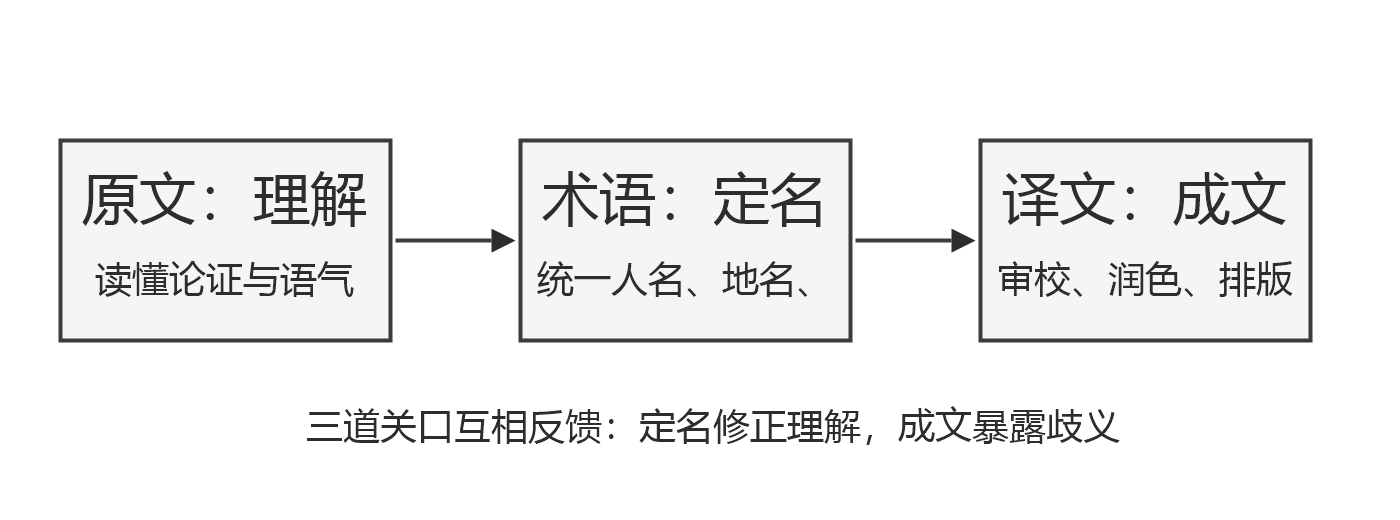
\includegraphics[width=0.72\textwidth]{figures/fig1-1.png}
  \caption{翻译流程中的三道关口：理解、定名、成文。}
  \label{fig:translation-gates}
  \figsource{示意图，由工作区模板生成。}
\end{figure}

如图 \ref{fig:translation-gates} 所示，三道关口并非线性通过：定名会反过来修正理解，成文又会暴露此前未察觉的歧义。因此，初译、审校、润色必须分开进行，不能指望一遍完成。

\section{术语与注释}

术语的一致性不是排版问题，而是理解问题。同一原文词在不同章节被译成不同中文，通常说明译者对该词的理解尚未稳定；反过来，强行统一一个多义词，也会让译文在某个语境里失真。可行的做法是：在 \texttt{glossary/terms.csv} 中记录定名、语境与禁用变体，由脚本在全书范围检查，而不是靠记忆。

原书脚注必须全部译出。脚注往往不是装饰，而是作者与同行对话的痕迹；删掉脚注，等于删掉论证的一部分。\footnote{示例原注：此处模拟原书脚注的排印方式，编号与正文对应。}译者注则用来处理另一种情况：原文的预设对中文读者不成立，或双关无法保留。两者都出现在页脚，但文本上必须可区分。

\begin{table}[htbp]
  \centering
  \caption{三类注释的处理方式}
  \label{tab:notes}
  \begin{tabular}{@{}lll@{}}
    \toprule
    类型 & 标记 & 处理原则 \\
    \midrule
    原书脚注 & \texttt{\textbackslash footnote} & 全译，不改编号关系 \\
    译者注 & \texttt{\textbackslash zhu} & 说明背景、双关、译名理由 \\
    原文夹注 & 括号 & 原样保留，不改成脚注 \\
    \bottomrule
  \end{tabular}
\end{table}

翻译的限度，说到底不是语言的限度，而是译者愿意在多大程度上贴近原文、又愿意在多大程度上为读者负责。这两件事并不矛盾；矛盾的是以为可以只做其中一件。

\chapter{第二示例章}
\label{ch:02}

本章用于演示章文件的最小结构：一个章标题、若干节、正文、脚注与图。实际项目中，每章一个文件，文件名与原文章号对应。

\section{章节文件约定}

章节文件只包含正文，不写导言区，不写 \verb|\begin{document}|。标题用 \verb|\chapter|，节用 \verb|\section|；不要手写“第一章”，编号由模板自动生成。

\section{与原文对齐}

段落与原文保持一一对应。若中文需要合并或拆分段落，应在 \texttt{notes/decisions.md} 中记录位置与理由，便于审校时对照。

跨章引用用标签，不用固定数字：

\begin{quote}
详见第 \ref{ch:01} 章关于术语一致性的讨论。
\end{quote}

这样增删章节后，编号与交叉引用会自动更新。

   % 自动生成：chapters/*.tex 的自然排序列表

% ---------------- 后置部分 ----------------
\backmatter
\chapter*{术语与人名对照表}
\addcontentsline{toc}{chapter}{术语与人名对照表}
\markboth{术语与人名对照表}{术语与人名对照表}

本表由 \texttt{scripts/prepare.py} 根据 \texttt{glossary/terms.csv} 自动生成。尚未最终定名的条目以“（暂定）”标出；候选词条见候选表 \texttt{glossary/\allowbreak candidates.csv}，不进入成书。

\vspace{0.8em}
% 由 scripts/prepare.py 从 glossary/terms.csv 生成，请勿手改
\begingroup
\small
\renewcommand{\arraystretch}{1.28}
\begin{longtable}{@{}p{0.30\textwidth}p{0.25\textwidth}p{0.36\textwidth}@{}}
\toprule
\textbf{原文} & \textbf{译名} & \textbf{备注} \\
\midrule
\endfirsthead
\toprule
\textbf{原文} & \textbf{译名} & \textbf{备注（续）} \\
\midrule
\endhead
\bottomrule
\endlastfoot
\multicolumn{3}{@{}l}{\sffamily\bfseries 术语} \\[2pt]
fidelity & 忠实 & 示例条目；视语境可分“信息忠实/语气忠实” \\
performativity & 述行性 & 示例条目；Austin 用语 \\
\addlinespace[4pt]
\end{longtable}
\endgroup


\IfFileExists{backmatter/bibliography.tex}{\chapter*{参考文献}
\addcontentsline{toc}{chapter}{参考文献}
\markboth{参考文献}{参考文献}

\IfFileExists{generated/bibliography.tex}
  {%
   \begingroup
   \small
   \setlength{\parindent}{0pt}
   \setlength{\parskip}{0.35em}
   \raggedright
   \sloppy
   \input{generated/bibliography}
   \endgroup
  }
  {%
   \begin{flushleft}
   \small
   尚无参考文献数据。将原文参考文献放入 \texttt{source/backmatter/bibliography.md}，构建时会由 \texttt{scripts/backmatter.py} 自动生成。
   \end{flushleft}
  }
}
\IfFileExists{backmatter/index.tex}{\chapter*{索引}
\addcontentsline{toc}{chapter}{索引}
\markboth{索引}{索引}

\IfFileExists{generated/index.tex}
  {%
   \begingroup
   \small
   \setlength{\parindent}{0pt}
   \begin{multicols}{2}
   \input{generated/index}
   \end{multicols}
   \endgroup
  }
  {%
   \begin{flushleft}
   \small
   尚无索引数据。将原文索引放入 \texttt{source/backmatter/index.md}，构建时会由 \texttt{scripts/backmatter.py} 自动生成。
   \end{flushleft}
  }
}
\chapter*{译后记}
\addcontentsline{toc}{chapter}{译后记}
\markboth{译后记}{译后记}

\begin{flushleft}

（此处写译后记：翻译缘起、版本选择、术语取舍、致谢。）

\vspace{0.8em}
本译本依据 \textit{\booktitleoriginal} 译出。翻译过程中参考了相关研究文献与通行译名；凡有争议之处，已在译者注中说明。

\vspace{1.2em}
\hfill 译者\\
\hfill \bookyear 年
\end{flushleft}


\end{document}
